\documentclass[letterpaper,11pt,twoside]{article}
\usepackage{graphicx} % Required for inserting images
\usepackage[table,xcdraw,dvipsnames]{xcolor}
\usepackage{amsmath,amsfonts,amssymb,amsthm}
\usepackage{listings}
\usepackage{lipsum}
\usepackage{hyperref}
\usepackage{enumitem}

\usepackage{tikz}
\usepackage[siunitx, RPvoltages]{circuitikz}
\usetikzlibrary{3d}
\usepackage{comment}
\usepackage{caption,subcaption}
\usepackage{pgfplots}
\usepackage{dsfont}
\pgfplotsset{compat=newest} % or a newer version if available
\usepgfplotslibrary{groupplots}
\usetikzlibrary{pgfplots.groupplots}
\usetikzlibrary{shapes.geometric, arrows}
\tikzstyle{arrow} = [->,>=stealth,shorten >=2pt]
\newcommand{\re}[1]{\text{Re}\left(#1\right)}
\newcommand{\im}[1]{\text{Im}\left(#1\right)}
\newcommand{\bA}{\bm{A}}
\newcommand{\bB}{\bm{B}}
\newcommand{\bC}{\bm{C}}
\newcommand{\bE}{\bm{E}}
\newcommand{\E}{\mathcal{E}}
\newcommand{\bH}{\bm{H}}
\newcommand{\bD}{\bm{D}}
\newcommand{\bO}{\bm{0}}
\newcommand{\br}{\bm{r}}
\newcommand{\bk}{\bm{k}}
\newcommand{\bh}{\bm{h}}
\newcommand{\bR}{\bm{R}}
\newcommand{\hA}{\hat{A}}
\newcommand{\hB}{\hat{B}}
\newcommand{\hC}{\hat{C}}
\newcommand{\hU}{\hat{U}}
\newcommand{\ha}{\hat{a}}
\newcommand{\hb}{\hat{b}}
\newcommand{\hc}{\hat{c}}
\newcommand{\hn}{\hat{n}}
\newcommand{\hH}{\hat{H}}
\newcommand{\hN}{\hat{N}}
\newcommand{\hr}{\bm{\hat{r}}}
\newcommand{\hbE}{\hat{\bm{E}}}
\newcommand{\hx}{\hat{x}}
\newcommand{\hsigma}{\hat{\sigma}}
\newcommand{\hX}{\hat{X}}
\newcommand{\hI}{\hat{I}}
\newcommand{\hp}{\hat{p}}
\newcommand{\hP}{\hat{P}}
\newcommand{\hS}{\hat{S}}
\newcommand{\hD}{\hat{D}}
\newcommand{\hy}{\hat{y}}
\newcommand{\hrho}{\hat{\rho}}
\newcommand{\hz}{\hat{z}}
\newcommand{\laplace}[1]{\mathscr{L}\left[#1\right]}
\newcommand{\ilaplace}[1]{\mathscr{L}^{-1}\left[#1\right]}
\newcommand{\fourier}[1]{\mathscr{F}\left[#1\right]}
\newcommand{\Tr}[1]{\text{Tr}\left[#1\right]}
\newcommand{\ifourier}[1]{\mathscr{F}^{-1}\left[#1\right]}
\newcommand{\ket}[1]{\left|#1\right\rangle}
\newcommand{\bra}[1]{\left\langle#1\right|}
\newcommand{\braket}[1]{\langle#1\rangle}
\newcommand{\D}{\mathcal{D}}
\usepackage{cancel}
\usepackage{bm}
\usepackage{fancyhdr}
\usepackage[utf8x]{inputenc}
\usepackage[T1]{fontenc}
\usepackage[margin=0.8in,top=1in,bottom=1in]{geometry}
%%%%%
\begin{filecontents*}{refs.bib}
@article{cohen1986quantum,
  title={Quantum mechanics, volume 1},
  author={Cohen-Tannoudji, Claude and Diu, Bernard and Laloe, Frank},
  journal={Quantum Mechanics},
  volume={1},
  pages={898},
  year={1986}
}
\end{filecontents*}
%
\newcommand{\institution}{University of Arizona}
\newcommand{\autor}{Nicolás Hernández Alegría}
\newcommand{\course}{OPTI 544 Quantum Optics}
\newcommand{\assignment}{Assignment 5}
%
\title{\textbf{\assignment}\\\course\\{\Large\institution}}
\author{\autor}
%\date{\today\\Total time: 12 hours}
%
\renewcommand{\sectionmark}[1]{\markright{#1}}
\fancypagestyle{mainstyle}{
    \fancyhf{} % Clear all header and footer fields
    \fancyfoot[C]{\thepage}
    \fancyhead[LE,RO]{\course} % Section name on odd pages
    \fancyhead[LO,RE]{\assignment}
    % Optional: Thin rules
    \renewcommand{\headrulewidth}{0pt} % Header rule
    \renewcommand{\footrulewidth}{0pt} % No footer rule
}
%
\begin{document}

\pagestyle{mainstyle}
\maketitle
%%
\section*{Exercise 1}
\begin{enumerate}[itemsep=0pt,topsep=0pt,parsep=0pt,label=\alph*)]
  \item The eigenvalues $E_\pm$ are:
  \begin{align*}
    |IE_\pm-\tilde{H}_{\mathrm{eff}}|&=0\\
    \left|\begin{bmatrix}
      E_\pm&0\\0&E_\pm
    \end{bmatrix}-\hbar\begin{bmatrix}
      -\Delta_L/2&\Omega/2\\\Omega^*/2&\Delta_L/2
    \end{bmatrix}\right|&=\\
    \begin{vmatrix}
    \frac{2E_\pm+\hbar\Delta_L}{2}&-\frac{\hbar\Omega}{2}\\
    -\frac{\hbar\Omega^*}{2}&\frac{2E_\pm-\hbar\Delta_L}{2}
    \end{vmatrix}&=\\
    (2E_\pm+\hbar\Delta_L)(2E_\pm-\hbar\Delta_L)-\hbar^2|\Omega|^2&=0\\
    4E_\pm^2-\hbar^2\Delta_L^2-\hbar^2|\Omega|^2&=\\
    E_\pm&=\pm\frac{\hbar}{2}\sqrt{\Delta_L^2+|\Omega|^2}=\pm\frac{\hbar\Omega_R}{2}.
  \end{align*}
  The eigenvectors $v_\pm$ are
  \begin{align*}
    \tilde{H}_{\mathrm{eff}}v_\pm&=E_\pm v_\pm\\
    \hbar\begin{bmatrix}
      -\Delta_L/2&\Omega/2\\\Omega^*/2&\Delta_L/2
    \end{bmatrix}\begin{bmatrix}
      v_1\\v_2
    \end{bmatrix}&=\pm\frac{\hbar\Omega_R}{2}\begin{bmatrix}
      v_1\\v_2
    \end{bmatrix}\\
    \begin{bmatrix}
      -\frac{\Delta_L}{2}v_1+\frac{\Omega}{2}v_2\\
      \frac{\Omega^*}{2}v_1+\frac{\Delta_L}{2}v_2
    \end{bmatrix}&=\begin{bmatrix}
      \pm\frac{\Omega_R}{2}v_1\\\pm\frac{\Omega_R}{2}v_2
    \end{bmatrix}\longrightarrow v_2=\frac{\Delta_L\pm\Omega_R}{\Omega}v_1\Longrightarrow v_\pm=\begin{bmatrix}
      1\\\frac{\Delta_L\pm\Omega_R}{\Omega}
    \end{bmatrix},
  \end{align*}
  or, by normalizing,
  \begin{align*}
    v_\pm=\frac{1}{\sqrt{2\Omega_R(\Omega_R\pm\Delta_L)}}\begin{bmatrix}
        \Omega\\\Delta_L\pm\Omega_R
      \end{bmatrix}=\frac{1}{N_\pm}\begin{bmatrix}
        \Omega\\\Delta_L\pm\Omega_R
      \end{bmatrix}.
  \end{align*}
  The eigenvector matrix is:
  \begin{align*}
    S=\begin{bmatrix}
      |&|\\
      v_+&v_-\\
      |&|
    \end{bmatrix}=\begin{bmatrix}
      \Omega/N_+&\Omega/N_-\\
      (\Delta_L+\Omega_R)/N_+&(\Delta_L-\Omega_R)/N_-
    \end{bmatrix}=V^{-1}.
  \end{align*}
  Then,
  \begin{align*}
    S^{-1}\tilde{H}_{\mathrm{eff}}S&=\hbar\begin{bmatrix}
      \frac{\Omega}{N_+}&\frac{\Omega}{N_-}\\
      \frac{\Delta_L+\Omega_R}{N_+}&\frac{\Delta_L-\Omega_R}{N_-}
    \end{bmatrix}^{-1}\begin{bmatrix}
      -\Delta_L/2&\Omega/2\\\Omega^*/2&\Delta_L/2
    \end{bmatrix}\begin{bmatrix}
      \frac{\Omega}{N_+}&\frac{\Omega}{N_-}\\
      \frac{\Delta_L+\Omega_R}{N_+}&\frac{\Delta_L-\Omega_R}{N_-}
    \end{bmatrix}\\
    &=\frac{-\hbar N_+N_-}{2\Omega\Omega_R}\begin{bmatrix}
      \frac{\Delta_L-\Omega_R}{N_-}&-\frac{\Omega}{N_-}\\-\frac{\Delta_L+\Omega_R}{N_+}&\frac{\Omega}{N_+}
    \end{bmatrix}\begin{bmatrix}
      -\Delta_L/2&\Omega/2\\\Omega^*/2&\Delta_L/2
    \end{bmatrix}\begin{bmatrix}
      \frac{\Omega}{N_+}&\frac{\Omega}{N_-}\\
      \frac{\Delta_L+\Omega_R}{N_+}&\frac{\Delta_L-\Omega_R}{N_-}
    \end{bmatrix}\\
    &=\frac{-\hbar N_+N_-}{4\Omega\Omega_R}\begin{bmatrix}
      \frac{\Delta_L-\Omega_R}{N_-}&-\frac{\Omega}{N_-}\\-\frac{\Delta_L+\Omega_R}{N_+}&\frac{\Omega}{N_+}
    \end{bmatrix}\begin{bmatrix}
      \frac{\Omega_R\Omega}{N_+}&-\frac{\Omega_R\Omega}{N_-}\\\frac{|\Omega|^2+\Delta_L^2+\Delta_L\Omega_R}{N_+}&\frac{|\Omega|^2+\Delta_L^2-\Delta_L\Omega_R}{N_-}
    \end{bmatrix}\\
    &=-\frac{\hbar N_+N_-}{4\Omega\Omega_R}\begin{bmatrix}
      \frac{-2\Omega\Omega^2_R}{N_+N_-}&0\\0&\frac{2\Omega\Omega^2_R}{N_+N_-}
    \end{bmatrix}\\
    S^{-1}\tilde{H}_{\mathrm{eff}}S&=\begin{bmatrix}
      \frac{\hbar\Omega_R}{2}&0\\0&-\frac{\hbar\Omega_R}{2}
    \end{bmatrix}=\begin{bmatrix}
      E_+&0\\0&E_-
    \end{bmatrix},
  \end{align*}
  confirming the correct eigenmodes. Also we need $S^-1$ for next parts:
  \begin{align*}
    V=S^{-1}=\frac{-N_+N_-}{2\Omega\Omega_R}\begin{bmatrix}
      \frac{\Delta_L-\Omega_R}{N_-}&-\frac{\Omega}{N_-}\\-\frac{\Delta_L+\Omega_R}{N_+}&\frac{\Omega}{N_+}
    \end{bmatrix}.
  \end{align*}
  \item The graph if $E_\pm$ versus $\Delta_L$ is shown below.
  \begin{figure}[htbp]
    \centering
    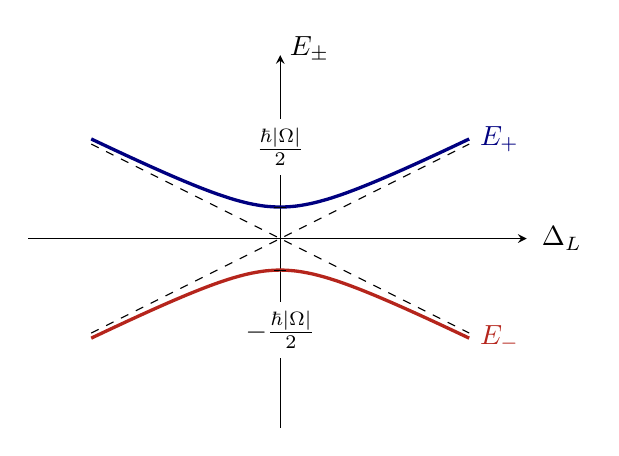
\begin{tikzpicture}[scale=.8]
      \def\Om{1}
      \draw[arrow](-4,0)--(4,0)node[right]{$\Delta_L$};
      \draw[arrow](0,-3)--(0,3)node[right]{$E_\pm$};
      \draw[domain=-3:3,smooth,variable=\x,NavyBlue,very thick]plot({\x},{(1/2)*sqrt( (\x*\x)+\Om*\Om)})node[right]{$E_+$};
      \draw[domain=-3:3,smooth,variable=\x,BrickRed,very thick]plot({\x},{-(1/2)*sqrt( (\x*\x)+\Om*\Om)})node[right]{$E_-$};
      \draw[](.1,.5)--(-.1,.5)(0,1)node[above,fill=white]{$\frac{\hbar|\Omega|}{2}$}(.1,-.5)--(-.1,-.5)(0,-1)node[below,fill=white]{$-\frac{\hbar|\Omega|}{2}$};
      \draw[dashed](-3,-1.5)--(3,1.5)(-3,1.5)--(3,-1.5);
    \end{tikzpicture}
    \caption{Phase space of the squeezed displaced state for $r=0.6$.}
  \end{figure}
  \item When diagonalizing I have two basis 
  \begin{align*}
    [\tilde{H}_{\mathrm{eff}}]_{\{\ket{e},\ket{g}\}}\xrightarrow{\text{Diagonalization}}[\tilde{H}_{\mathrm{eff}}]_{\{\ket{+},\ket{-}\}},
  \end{align*}
  they are related through 
  \begin{align*}
    \bC_{\{\ket{+},\ket{-}\}}=V\bm{c}_{\{\ket{e},\ket{g}\}},\quad \bC=\begin{bmatrix}
      C_+\\C_-
    \end{bmatrix},\;\bm{c}=\begin{bmatrix}
      \tilde{c}_e\\\tilde{c}_g
    \end{bmatrix}.
  \end{align*}
  The dressed states $\ket{\pm}$ in the bare basis are related through the eigenvector matrix $V^{-1}$:
  \begin{align*}
    [\ket{+}\;\ket{-}]=[\ket{e}\;\ket{g}]V^{-1}\longrightarrow\ket{\pm}=\frac{1}{N_\pm}[\Omega\ket{e}+(\Delta_L\pm\Omega_R)\ket{g}],\quad N_\pm=\sqrt{2\Omega_R(\Omega_R\pm\Delta_L)}.
  \end{align*}
  We can get a standard form of the dressed states starting from the coefficient $c_e$ and $c_g$:
  \begin{align*}
    c^2_e&=\frac{\Omega^2}{2\Omega_R(\Omega_R+\Delta_L)}=\frac{(\Omega_R+\Delta_L)(\Omega_R-\Delta_L)}{2\Omega_R(\Omega_R+\Delta_L)}=\frac{\Omega_R-\Delta_L}{2\Omega_R}=\frac{1-\Delta_L/\Omega_R}{2},\\
    c^2_g&=\frac{(\Omega_R+\Delta_L)^2}{2\Omega_R(\Omega_R+\Delta_L)}=\frac{\Omega_R+\Delta_L}{2\Omega_R}=\frac{1+\Delta_L/\Omega_R}{2}.
  \end{align*}
  If we equate the last result of $c_e^2$ to $\cos^2(\theta)$, we get:
  \begin{align*}
    \cos^2\theta=\frac{1+\cos2\theta}{2}=\frac{1-\Delta_L/\Omega_R}{2}\Longrightarrow\cos2\theta=-\frac{\Delta_L}{\Omega_R}.
  \end{align*}
  Then,
  \begin{align*}
    \cos^22\theta+\sin^22\theta=1\longrightarrow\sin2\theta=\sqrt{1-\Delta_L^2/\Omega_R^2}=\sqrt{\frac{\Omega_R^2-\Delta_L^2}{\Omega_R^2}}=+\frac{\Omega}{\Omega_R}.
  \end{align*}
  Using both result we get
  \begin{align*}
    \tan2\theta=\frac{\sin2\theta}{\cos2\theta}=\frac{\Omega/\Omega_R}{-\Delta_L/\Omega_R}=-\frac{\Omega}{\Delta_L}.
  \end{align*}
  Therefore,
  \begin{align*}
    \ket{\pm}=\cos\theta\ket{e}+\sin\theta\ket{g},\quad\tan2\theta=-\frac{\Omega}{\Delta_L},
  \end{align*}
  and doing the same process we get:
  \begin{align*}
    \ket{-}=-\sin\theta\ket{e}+\cos\theta\ket{g}.
  \end{align*}
  The detuning $\Delta_L$ change the amplitude of the bare states. In particular, 
  \begin{align*}
    \ket{\pm}=\begin{cases}
      \ket{\substack{g\\e}},&\Delta_L\ll0\\
      \frac{1}{\sqrt{2}}[\ket{e}\pm\ket{g}],&\Delta_L=0\\
      \ket{\substack{e\\g}},&\Delta_L\gg0
    \end{cases}.
  \end{align*}
  \item For $\Delta_L=0$, the dressed states take the form:
  \begin{align*}
    \ket{\pm}=\frac{1}{\sqrt{2}}[\ket{e}\pm\ket{g}].
  \end{align*}
  If the state of the atom is $\ket{\Psi(t)}$, the given initial state is 
  \begin{align*}
    \ket{\Psi(0)}=\frac{1}{\sqrt{2}}[\ket{e}+\ket{g}]=\ket{+}.
  \end{align*}
  Its evolution in general, will be stationary because $\ket{+}$ is one eigenstate of the Hamiltonian:
  \begin{align*}
    \ket{\Psi(t)}=e^{-i\Omega t/2}\ket{+}.
  \end{align*} 
  At $t=\pi/\Omega$, we have:
  \begin{align*}
    \ket{\Psi(\pi/\Omega)}=e^{-i\pi/2}\ket{+}=-i\ket{+}=\frac{-i}{\sqrt{2}}[\ket{e}+\ket{g}].
  \end{align*}
\end{enumerate}


\section*{Exercise 2}
\begin{enumerate}[itemsep=0pt,topsep=0pt,parsep=0pt,label=\alph*)]
  \item The effective Hamiltonian can be expressed in terms of the Pauli matrices:
  \begin{align*}
    \tilde{H}_{\mathrm{eff}}=\hbar\begin{bmatrix}
      -\Delta_L/2&\Omega/2\\\Omega^*/2&\Delta_L/2
    \end{bmatrix}=h_x\begin{bmatrix}
      0&1\\1&0
    \end{bmatrix}+h_y\begin{bmatrix}
      0&-i\\i&0
    \end{bmatrix}+h_z\begin{bmatrix}
      1&0\\0&-1
    \end{bmatrix}+h_1\begin{bmatrix}
      1&0\\0&1
    \end{bmatrix}
  \end{align*}
  By equating each element of the matrix we have four equations:
  \begin{align*}
    \left.\begin{array}{rl}
      (1):&h_z+h_1=\frac{-\hbar\Delta_L}{2}\\
      (2):&h_x-ih_y=\frac{\hbar\Omega}{2}\\
      (3):&h_x+ih_y=\frac{\hbar\Omega^*}{2}\\
      (4):&h_1-h_z=\frac{\hbar\Delta_L}{2}
    \end{array}\right\rfloor
  \end{align*}
  By playing with those, we have the following results:
  \begin{align*}
    &(1)+(4)\Longrightarrow h_1=0,\quad (2)+(3)\Longrightarrow h_x=\frac{\hbar\re{\Omega}}{2},\\
    &\quad (1)-(4)\Longrightarrow h_z=-\frac{\hbar\Delta_L}{2},\quad(2)-(3)\Longrightarrow h_y=-\frac{\hbar\im{\Omega}}{2}.
  \end{align*}
  Pauli matrices commute each other, so the evolution operator can be written as a separate exponential:
  \begin{align*}
    e^{-\frac{i\tilde{H}_{\mathrm{eff}}t}{\hbar}}=e^{-\frac{i[h_x\hsigma_x+h_y\hsigma_y+h_z\hsigma_z]t}{\hbar}}=e^{-\frac{i\re{\Omega}t}{2}}e^{\frac{i\Delta_Lt}{2}}e^{\frac{i\im{\Omega}t}{2}}.
  \end{align*}
  The vector precession is:
  \begin{align*}
    \bh=\frac{\hbar\re{\Omega}}{2}\bm{x}-\frac{\hbar\im{\Omega}}{2}\bm{y}-\frac{\hbar\Delta_L}{2}\bm{z}.
  \end{align*}
  \item Assuming $\Omega$ real, the effective Hamiltonian is:
  \begin{align*}
    \tilde{H}_{\mathrm{eff}}=\frac{\hbar}{2}\bm{\Omega}_{\mathrm{eff}}\cdot\bm{\sigma}+\mathds{I}=\frac{\hbar}{2}\left[\Omega\hsigma_x-\Delta_L\hsigma_z\right],\quad\bm{\Omega}_{\mathrm{eff}}=(\Omega,0,-\Delta_L).
  \end{align*}
  The rotation in the Bloch sphere is governed by the following expression:
  \begin{align*}
    \br(t)=\br(0)\cos(\Omega_{\mathrm{eff}}t)+(\hat{\Omega}_{\mathrm{eff}}\times\br(0))\sin(\Omega_{\mathrm{eff}}t)+\hat{\Omega}_{\mathrm{eff}}
    (\hat{\Omega}_{\mathrm{eff}}\cdot\br(0))[1-\cos(\Omega_{\mathrm{eff}}t)].
  \end{align*}
  For each case, with the initial atom in the ground state $\br(0)=(0,0,-1)$, we have 
  \begin{align*}
    \Delta_L=0:&\qquad\bm{\Omega}_{\mathrm{eff}}=(\Omega,0,0),\quad\hat{\Omega}_{\mathrm{eff}}=(1,0,0),\quad\Omega_{\mathrm{eff}}=\Omega,\\
    \Delta_L=\Omega:&\qquad\bm{\Omega}_{\mathrm{eff}}=(\Omega,0,-\Omega),\quad\hat{\Omega}_{\mathrm{eff}}=\frac{1}{\sqrt{2}}(1,0,-1),\quad\Omega_{\mathrm{eff}}=\sqrt{2}\Omega.
  \end{align*}
  The rotation vector for the first case is:
  \begin{align*}
    \br(t)&=(0,0,-1)\cos(\Omega t)+[(1,0,0)\times(0,0,-1)]\sin(\Omega t)+(1,0,0)[(1,0,0)\cdot(0,0,-1)][1-\cos(\Omega t)]\\
    &=(0,0,-1)\cos(\Omega t)+(0,1,0)\sin(\Omega t)\\
    \br(t)&=[0,\sin(\Omega t),-\cos(\Omega t)].
  \end{align*}
  For the second is:
  \begin{align*}
    \br(t)=&(0,0,-1)\cos(\sqrt{2}\Omega t)+\frac{1}{\sqrt{2}}[(1,0,-1)\times(0,0,-1)]\sin(\sqrt{2}\Omega t)\\
    &+\frac{1}{2}(1,0,-1)[(1,0,-1)\cdot(0,0,-1)][1-\cos(\sqrt{2}\Omega t)]\\
    =&(0,0,-1)\cos(\sqrt{2}\Omega t)+\frac{1}{\sqrt{2}}(0,1,0)\sin(\sqrt{2}\Omega t)+\frac{1}{2}(1,0,-1)[1-\cos(\sqrt{2}t)]\\
    \br(t)=&\left(\frac{1-\cos(\sqrt{2}\Omega t)}{2},\frac{\sin(\sqrt{2}\Omega t)}{\sqrt{2}},-\frac{1+\cos(\sqrt{2}\Omega t)}{2}\right).
  \end{align*}
\end{enumerate}

\begin{figure}[htbp]
  \centering
  \begin{subfigure}{.45\columnwidth}
    \centering
    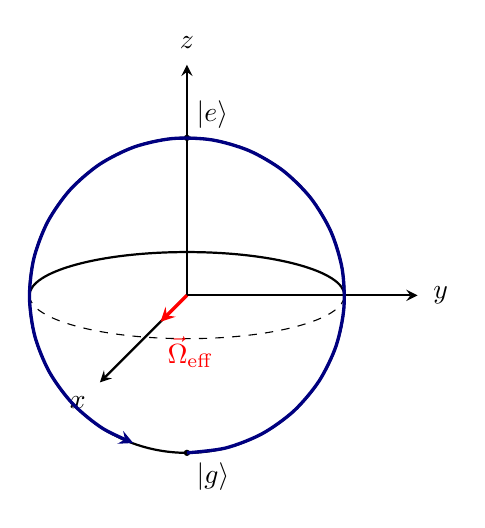
\begin{tikzpicture}[scale=1]
    \def\R{2.0}
    \coordinate (O) at (0,0);
    %\shade[ball color=gray!10, opacity=0.25] (O) circle (\R);
    \draw[thick](O)circle(\R);
    \draw[dashed] (-\R,0) arc[start angle=180,end angle=360,x radius=\R,y radius=0.55];
    \draw[thick]  (\R,0) arc[start angle=0,end angle=180,x radius=\R,y radius=0.55];
    %(y,z,x)
    \draw[arrow,thick] (0,0,0) -- (0,1.5*\R,0) node[above] {$z$};
    \draw[arrow,thick] (0,0,0) -- (1.5*\R,0,0) node[right] {$y$};
    \draw[arrow,thick] (0,0,0) -- (0,0,1.5*\R) node[below left] {$x$};
    \fill (0,\R) circle (0.04) node[above right] {$\ket{e}$};
    \fill (0,-\R) circle (0.04) node[below right] {$\ket{g}$};
    % effective axis for case 2
    \draw[red,arrow,very thick](0,0)--(0,0,1)node[below right] {$\vec\Omega_{\rm eff}$};
    \draw[domain=0:{1.9*pi},smooth,variable=\x,NavyBlue,very thick,arrow]
    plot({\R*sin(deg(\x))},{-\R*cos(deg(\x))},{0});
    \end{tikzpicture}
    \caption{$\Delta_L=0$}
  \end{subfigure}
  \hfill
  \begin{subfigure}{.45\columnwidth}
    \centering
    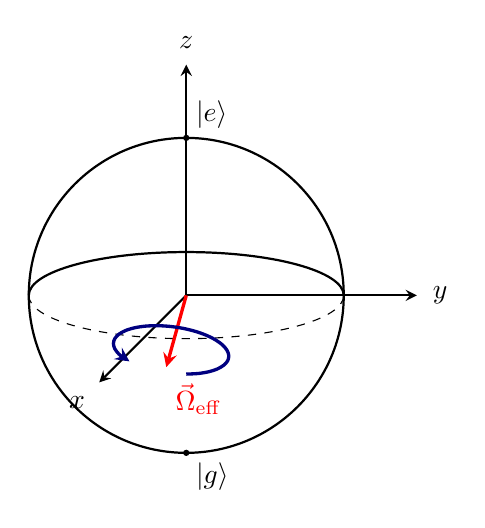
\begin{tikzpicture}[scale=1]
    \def\R{2.0}
    \coordinate (O) at (0,0);
    %\shade[ball color=gray!10, opacity=0.25] (O) circle (\R);
    \draw[thick](O)circle(\R);
    \draw[dashed] (-\R,0) arc[start angle=180,end angle=360,x radius=\R,y radius=0.55];
    \draw[thick]  (\R,0) arc[start angle=0,end angle=180,x radius=\R,y radius=0.55];
    %(y,z,x)
    \draw[arrow,thick] (0,0,0) -- (0,1.5*\R,0) node[above] {$z$};
    \draw[arrow,thick] (0,0,0) -- (1.5*\R,0,0) node[right] {$y$};
    \draw[arrow,thick] (0,0,0) -- (0,0,1.5*\R) node[below left] {$x$};
    \fill (0,\R) circle (0.04) node[above right] {$\ket{e}$};
    \fill (0,-\R) circle (0.04) node[below right] {$\ket{g}$};
    % effective axis for case 2
    \draw[red,arrow,very thick](0,0)--(0,{-1/sqrt(2)},{1/sqrt(2)})node[below right] {$\vec\Omega_{\rm eff}$};
    \draw[domain=0:{1.2*pi},smooth,variable=\x,NavyBlue,very thick,arrow]
    plot({sin(deg(sqrt(2)*\x))/sqrt(2)},{-(1+cos(deg(sqrt(2)*\x)))/2},{(1-cos(deg(sqrt(2)*\x)))/2});
    \end{tikzpicture}
    \caption{$\Delta_L=\Omega$}
  \end{subfigure}
\end{figure}


%\clearpage
%\nocite{*}
%\bibliographystyle{plain}   % or unsrt, alpha, apalike, etc.
%\bibliography{refs}






\end{document}
